\let\negmedspace\undefined
\let\negthickspace\undefined
%\RequirePackage{amsmath}
\documentclass[journal,12pt,twocolumn]{IEEEtran}
 \usepackage[utf8]{inputenc}
 \usepackage{graphicx}
 \usepackage{amsmath}
 \usepackage{mathrsfs}
\usepackage{txfonts}
\usepackage{stfloats}
\usepackage{bm}
\usepackage{cite}
\usepackage{cases}
\usepackage{subfig}
 \usepackage{amsfonts}
 \usepackage{amssymb}
 \usepackage{enumitem}
\usepackage{mathtools}
\usepackage{tikz}
\usepackage{circuitikz}
\usepackage{verbatim}
\usepackage[breaklinks=false,hidelinks]{hyperref}
\usepackage{listings}
\usepackage{calc}
\usepackage{float}
\usepackage{longtable}
\usepackage{multirow}
\usepackage{multicol}
\usepackage{color}
\usepackage{array}
\usepackage{hhline}
\usepackage{ifthen}
\usepackage{chngcntr}

\newcommand{\BEQA}{\begin{eqnarray}}
\newcommand{\EEQA}{\end{eqnarray}}
\newcommand{\define}{\stackrel{\triangle}{=}}
\bibliographystyle{IEEEtran}
%\bibliographystyle{ieeetr}
\def\inputGnumericTable{}

\let\vec\mathbf

\providecommand{\pr}[1]{\ensuremath{\Pr\left(#1\right)}}
\providecommand{\sbrak}[1]{\ensuremath{{}\left[#1\right]}}
\providecommand{\lsbrak}[1]{\ensuremath{{}\left[#1\right.}}
\providecommand{\rsbrak}[1]{\ensuremath{{}\left.#1\right]}}
\providecommand{\brak}[1]{\ensuremath{\left(#1\right)}}
\providecommand{\lbrak}[1]{\ensuremath{\left(#1\right.}}
\providecommand{\rbrak}[1]{\ensuremath{\left.#1\right)}}
\providecommand{\cbrak}[1]{\ensuremath{\left\{#1\right\}}}
\providecommand{\lcbrak}[1]{\ensuremath{\left\{#1\right.}}
\providecommand{\rcbrak}[1]{\ensuremath{\left.#1\right\}}}
\providecommand{\res}[1]{\Res\displaylimits_{#1}}
\newcommand{\myvec}[1]{\ensuremath{\begin{pmatrix}#1\end{pmatrix}}}
\newcommand{\mydet}[1]{\ensuremath{\begin{vmatrix}#1\end{vmatrix}}}

\newcommand{\question}{\noindent \textbf{Question: }}
\newcommand{\solution}{\noindent \textbf{Solution: }}


\title{Assignment 4}
\author{Donal Loitam(AI21BTECH11009)}
\date{}
\begin{document}
% make the title area
\maketitle
\question \textbf{(CBSE CLASS 11 - Example 11)}\\
 A bag contains 9 discs of which 4 are red, 3 are blue and 2 are yellow.
The discs are similar in shape and size. A disc is drawn at random from the bag.
Calculate the probability that it will be:
\begin{enumerate}[label=(\roman{enumi})]
	\item red
	\item yellow
	\item blue
	\item not blue
	\item  either red or blue
\end{enumerate}
\solution
\begin{table}[ht!]
\begin{center}
		\normalsize \begin{tabular}{|c|c|c|c|c|c|}

\hline
\textbf{Color} & \textbf{No. of Discs} \\
\hline
  Red          &     $4$\\
\hline
  Yellow        &     $2$\\
\hline
  Blue          &     $3$\\
\hline
\textbf{Total}        &     $9$\\
\hline
\end{tabular}

		\vspace*{5pt}
		\caption{}
		\label{table:table1}
\end{center}	
	\end{table}\\
Let a random variable $X$ denote the outcome of the experiment such that:-
\begin{table}[ht!]
\begin{center}
		\normalsize \begin{tabular}{|c|c|c|c|c|c|}

\hline
\textbf{Event} & \textbf{Description} \\
\hline
  $X=0$          &     Drawn ball is Red\\
\hline
  $X=1$          &     Drawn ball is Yellow\\
  \hline
  $X=2$          &     Drawn ball is Blue\\
\hline
\end{tabular}

		\vspace*{5pt}
		\caption{}
		\label{table:table1}
\end{center}	
	\end{table}\\
	
\begin{enumerate}[label=(\roman{enumi})]
    \item $X = 0$ denotes the disc is red.
    \begin{align}
        \pr{X = 0} & = \frac{4}{9} 
	    \\
	    & = \fbox{0.444}
    \end{align}
    \item $X = 1$ denotes the disc is yellow.
    \begin{align}
        \pr{X = 1} & = \frac{2}{9} 
	    \\
	    & = \fbox{0.222}
    \end{align}
    \item $X = 2$ denotes the disc is blue.
    \begin{align}
        \pr{X = 2} & = \frac{3}{9} \\
        & = \frac{1}{3} \\
	    & = \fbox{0.333}
    \end{align}
    \item $X \not = 2$ denotes the disc is not blue, that is,
	$X \in \cbrak{0,1}$. Thus, the disc is either yellow or red.
    \begin{align}
        \pr{X \not = 2} & = \pr{X \in \cbrak{0,1}}
		\\
		& = \pr{X = 0} + \pr{X = 1}
		\\
		& =\frac{4+2}{9}
	    \\
	    & =\frac{2}{3}
	    \\
	    & = \fbox{0.667}
    \end{align}
    \item $X \in \cbrak{0,2}$ denotes the disc is either red or blue.
    \begin{align}
       \pr{X \in \cbrak{0,2}} & = \pr{X = 0} + \pr{X = 2}
		\\
		& =\frac{4+3}{9}
	    \\
	    & =\frac{7}{9}
	    \\
	    & = \fbox{0.778}
    \end{align}
\end{enumerate}
\begin{figure}[h] 
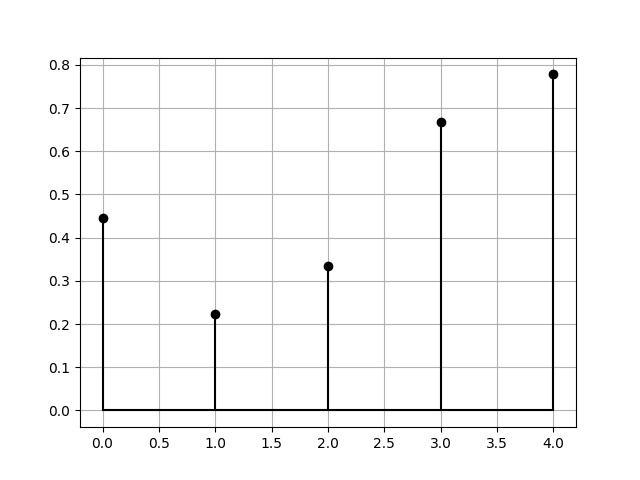
\includegraphics[width=\columnwidth] 
{assignment_4}
\caption{Plot of PMF using above data}
\label{fig:a}
\end{figure}
\end{document}
